\section{The ADF Software Library}
\label{s:library}
\thispagestyle{plain}

The ADF library is a hierarchical database system that is built around
the concept of a ``node''.
Each node contains information about itself and its ancestors and
possibly data (e.g., arrays, vectors, character strings, etc.).
Each of these nodes, in turn, can be connected to an arbitrary number of
children, each of which is itself a node.
In this system, an ADF node contains user-accessible information related
to identification, name, type, and amount of data associated with it,
and pointers to child nodes.
Basic nodal information includes:

\begin{itemize}
\item a unique ID (essentially a file location pointer)
\item a name (character string) used to describe the node and its data
\item a label (character string) an additional field used to describe the
      node and its data.
      It is analogous to, but not exactly the same as, the name.
\item information describing the type and amount of data
\item data
\item IDs of child nodes
\end{itemize}

There are no restrictions on the number of child nodes that a node can
have associated with it in the ADF database.
This structure allows the construction of a hierarchical database as
shown in \autoref{f:example} on p.~\pageref*{f:example}.
As illustrated in the figure, it is possible to reference nodes in a
second file (\textit{ADF\_File\_Two}) from the original file
(\textit{ADF\_File\_One}).
This is the concept of ``linking.''
\begin{figure}[!htb]
   \centering
   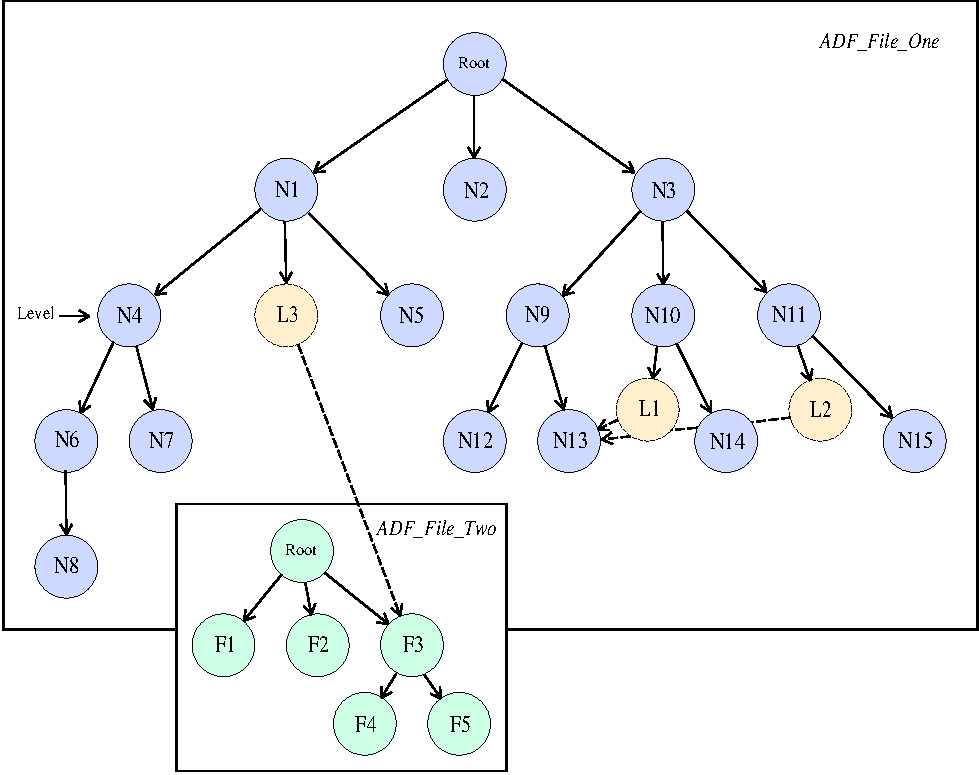
\includegraphics[width=6.0in]{adf_figure}
   \caption{Example Database Hierarchy of Nodes}
   \label{f:example}
\end{figure}

A node knows about itself and its children, but it does not know
anything about its parent.
This means that it is possible to traverse ``down'' the tree by making
queries about what lies below the current node, but it is not possible
to traverse ``up'' the tree by making queries about nodes above a given
node.
If it is desired to move back up the tree, the user must keep track of
that information.

All ADF files start with the root node, named ``ADF MotherNode''.
This node is created automatically when a new file is opened.
There is only one root node in an ADF file.

\subsection{ADF Node Attributes}
\label{s:node}

There is a single building block called a node (see \autoref{f:example})
used to construct the hierarchical structure.
Each node may have zero to many subnodes that are associated with it, as
well as its own data.
The following are a list of attributes accessible by the user for a node
in the ADF hierarchical database system.

\begin{Ventryi}{Number of Dimensions}
\item [Child Table]
      A table of file pointers and names for each of the node's
      children.
\item [Data]
      The data associated with a node.
\item [Data Type]
      A 32-byte character field, blank filled, case sensitive.
      Specifies the type of data (e.g., real, integer, complex)
      associated with this node.
      The supported data types are listed in \autoref{t:datatype}
      on p.~\pageref*{t:datatype}.

\begin{table}[htbp]
\centering
\caption[Data Types]{\textbf{Data Types}}
\label{t:datatype}
\begin{tabular}{l >{\quad}l}
\\ \hline\hline \\*[-2ex]
\bold{Data Type} & \bold{Notation}
\\*[1ex] \hline\hline \\*[-2ex]
No Data                   & \fort{MT} (i.e., eMpTy) \\
Integer 32                & \fort{I4} \\
Integer 64                & \fort{I8} \\
Unsigned Integer 32       & \fort{U4} \\
Unsigned Integer 64       & \fort{U8} \\
Real 32                   & \fort{R4} \\
Real 64                   & \fort{R8} \\
Complex 64                & \fort{X4} \\
Complex 128               & \fort{X8} \\
Character (unsigned byte) & \fort{C1} \\
Byte (unsigned byte)      & \fort{B1} \\
Link                      & \fort{LK}
\\*[1ex] \hline\hline
\end{tabular}
\end{table}

\item [Dimensions]
      An integer vector containing the number of elements within
      each dimension.
      For example, if the array \fort{A} was declared (using Fortran) as
      \fort{A(10,20)}, the Dimension vector would contain two entries
      (10,20).
\item [ID]
      A unique identifier to access a given node within a file.
      This field contains sufficient information for ADF to locate the
      node within a file.
      For any given node, the ID is generated only after the file it
      resides in has been opened by a program and the user requests
      information about the node.
      The ID is valid only within the program that opened the file and
      while that file is open.
      If the file is closed and reopened, the ID for any given node
      will be different.
      Within different programs, the node ID for the same node will be
      different.
      The ID is never actually written into a file.
\item [Label]
      A 32-byte character field.
      The rules for Labels are identical to those for Names.
      Unlike names, Labels do not have to be unique.
      The Label field was introduced to allow ``data typing'' similar to
      the ``typedef'' concept in C.
      Using the Label field in this way allows programs to know some
      additional information about the use of the node itself or its
      child nodes and to call specific subroutines to read the data or
      react in specific ways upon detection of the type.
\item [Name]
      A 32-byte character field.
      The names of child nodes directly attached to a parent node must
      be unique.
      For example, in \autoref{f:example}, all nodes directly attached
      to N3 must have unique names.
      When a request to create a new node is made, ADF checks the
      requested name against the other names of the child nodes of the
      specified parent.
      If the requested name is not unique, ADF returns an error.

      Legal characteristics of a name are a A-Z, a-z, 0-9, and special
      characters (ASCII values from 32 to 126, except for the forward
      slash ``/'' (ASCII number 47)).
      Names will be blank filled to 32 bytes; they are case sensitive.
      Leading blanks are discarded and trailing blanks are ignored,
      whereas internal blanks are significant.

      \emph{Note}: Names passed to ADF from C must have the null
      ``\textbackslash0'' character appended to them.
      Names returned from ADF through the C interface will have the
      null character appended to them.
      Therefore, C programs should allocate 33 bytes for any Name in
      order to accommodate the null character.

      Fortran programs can allocate 32 characters for Names.
      The Fortran interface takes care of adding or removing the null
      character as required.
\item [Names of Subnodes]
      A list of names of the subnodes (children) of a node.
      (This is the information contained in the child table.)
\item [Number of Dimensions]
      The dimensionality of the data.
      ADF views all data as an array and can handle from zero (i.e., no
      data) to 12 dimensions.
      A ``0'' is used if the data type is empty.
      Thus, a scalar is viewed as a vector with one dimension and
      length 1.
\item [Number of Subnodes]
      The number of child nodes directly attached to any given node.
      Each node can have zero or more child nodes directly associated
      with it.
\item [Pointer]
      An address, from the point of view of a programming language.
      Pointers are like jumps, leading from one part of the data
      structure to another.
\end{Ventryi}

\subsubsection{Data Type Definitions}

\begin{Ventryi}{Character}
\item [Structure]
      It is possible to define a ``structure'' in ADF similar to the way
      that ``struct'' is defined in the C programming language.
      ADF will treat each instance of the structure as a single
      instance of data.
      A structure is described by using a string.
      For example: ``\fort{I4,I4,R8,R4}''.

      \emph{Notes:}
      \begin{itemize}
      \item Structures can be only as complex as can be described in 32
            characters.
      \item This construct is not very portable; therefore, its use is
            highly discouraged.
      \end{itemize}
\item [Character]
      A character type is intended for ASCII-type character information.
      There may be different system architectures that use different
      representations for translating data.
      Byte data type should be used for pure byte or bit data usage.
\item [Precision]
      The \fort{R4} and \fort{R8} are single and double precision,
      respectively, on a 32-bit system architecture.
      On the Cray, single precision is \fort{R8} and double precision
      may be \fort{R8} or \fort{R16}, depending on the compile
      settings.
      ADF tracks the number of bits to guarantee precision.
\item [Link]
      A link is denoted by ``\fort{LK}'' in \autoref{t:datatype} on
      p.~\pageref*{t:datatype} and defines the linkage between nodes and
      subnodes.
      A link provides a mechanism for referring to a node that
      physically resides in a different part of the hierarchy or a
      different file.
      A link within ADF parallels a soft link in the UNIX operating
      system in that it does not guarantee that the referenced node
      exists.
      ADF will ``resolve'' the link only when information is requested
      about the linked node.
\end{Ventryi}

\subsection{Acquiring the Software and Documentation}

The ADF software is distributed as part of the CGNS Library, available
from SourceForge, at
\href{http://sourceforge.net/projects/cgns}{http://sourceforge.net/projects/cgns}.
This manual, as well as the other CGNS documentation, is available in
both HTML and PDF format from the CGNS documentation web site, at
\href{http://www.grc.nasa.gov/www/cgns/}{http://www.grc.nasa.gov/www/cgns/}.
